\documentclass[conference]{IEEEtran}
\IEEEoverridecommandlockouts
\usepackage{cite}
\usepackage{amsmath,amssymb,amsfonts}
\usepackage{algorithmic}
\usepackage{graphicx}
\usepackage{textcomp}
\usepackage{xcolor}
\usepackage{booktabs}
\usepackage{url}
\usepackage{microtype}

\begin{document}

\title{GodXplr: A High-Performance, Zero-Hydration Native Filesystem Management and Content Retrieval Architecture\\
\thanks{Submitted in partial fulfillment of the academic requirements for the Bachelor of Technology in Computer Science and Engineering.}
}

\author{\IEEEauthorblockN{Shreyansh Prasad}
\IEEEauthorblockA{\textit{Department of Computer Science and Engineering} \\
\textit{Netaji Subhas University of Technology (NSUT)}\\
New Delhi, India \\
Roll No: 2025UCS1708 \\
Email: shreyanshtrillion@gmail.com}
}

\maketitle

\begin{abstract}
Modern desktop file management shells and content retrieval engines frequently encounter notable performance bottlenecks, including elevated memory consumption, multi-second query latencies during recursive searches, and uncoordinated cloud-storage hydration stalls. Many consumer desktop managers rely on heavyweight web-wrapper runtimes or unvirtualized graphical frameworks that allocate discrete UI objects for every listed entity, resulting in high resource consumption. Furthermore, standard search indexers often incur substantial storage footprints or inadvertently trigger remote downloads of offline cloud placeholder files during background directory traversals.

This paper presents \textbf{GodXplr}, a native filesystem management and content retrieval architecture implemented in standard C++20 for the Windows platform. GodXplr integrates: (i) an asynchronous indexing subsystem utilizing bulk-buffered NTFS Master File Table (MFT) enumeration and real-time Update Sequence Number (USN) Journal tailing; (ii) an AVX2 SIMD-vectorized multi-needle substring filtering engine operating across 32 byte-wide lanes per 256-bit register; (iii) a memory-bounded, positionless inverted trigram content index; (iv) a file operation intent logging engine (\texttt{OperationJournal}) with startup recovery and partial transfer cleanup; (v) a cloud placeholder defense gate that intercepts Windows Cloud Filter API reparse tags to prevent unwanted remote file hydration; and (vi) a row-virtualized user interface implemented natively using the Win32 GDI API, projecting visible rows in $O(1)$ time relative to directory size, with double-buffered rendering and direct manipulation interaction dynamics.

Empirical evaluations demonstrate that GodXplr indexes 100,000 file entries in 54.92~ms with an average raw index payload density of 132.5 bytes per entry (13.25~MB total index payload; 23.9~MB overall application working set), sustains sub-millisecond query search latencies ($p_{50} = 655~\mu\text{s}$), achieves a $24.3\times$ process memory reduction compared to Windows 11 File Explorer under equivalent scale, and passes 100\% of an automated 28-suite integration test harness under MSVC \texttt{/W4 /WX}.
\end{abstract}

\begin{IEEEkeywords}
Filesystem Indexing, NTFS USN Journal, SIMD Vectorization, Inverted Trigram Index, Cloud Placeholders, UI Row Virtualization, Win32 GDI, File Operation Journaling.
\end{IEEEkeywords}

\section{Introduction}
The desktop filesystem shell serves as the primary interface between users and hierarchical secondary storage \cite{silberschatz_os}. Over the past three decades, rapid expansions in storage capacity, solid-state drive (SSD) throughput, and cloud synchronization networks have increased typical user data collections from thousands of local files to millions of heterogeneous entities distributed across local volumes, virtual network mounts, and cloud-backed synchronized directories (e.g., Microsoft OneDrive, Google Drive, Apple iCloud Drive).

Despite hardware advancements, modern desktop file managers (e.g., Windows File Explorer, macOS Finder) exhibit notable architectural limitations:
\begin{enumerate}
    \item \textbf{High Memory Overhead:} Contemporary GUI frameworks (such as WinUI 3, XAML Islands, and web-based wrappers) often require hundreds of megabytes of working memory for basic directory listings by instantiating discrete UI object wrappers for each item.
    \item \textbf{High Traversal Latency:} Traditional hierarchical file enumeration APIs (\texttt{FindFirstFileW} / \texttt{FindNextFileW}) perform sequential disk directory lookups. When querying millions of files, searches can take tens of seconds or cause responsiveness drops in the desktop shell.
    \item \textbf{Uncoordinated Cloud Storage Hydration:} Cloud-integrated filesystems represent remote non-cached files using reparse points. Standard search engines and thumbnail generators frequently access these files naively, triggering automated network downloads of large remote files, consuming network bandwidth and local disk storage.
    \item \textbf{Non-Journaled File Mutations:} Standard desktop file operations typically lack structured intent logging. A system interruption or process termination during a multi-gigabyte file migration can leave directories in inconsistent or partially transferred states.
\end{enumerate}

To address these engineering challenges, this paper presents \textbf{GodXplr}, an integrated native filesystem management and indexing architecture. Implemented in ISO C++20 with zero third-party GUI framework dependencies, GodXplr utilizes direct Win32 kernel control APIs, SIMD vector extensions, and memory-isolated viewport rendering to achieve low latency and minimal resource utilization.

\section{Problem Statement and Objectives}
The primary objective of GodXplr is to design, implement, and validate an integrated desktop file manager that balances visual responsiveness, query throughput, and memory consumption. Five technical goals guide the architecture:
\begin{itemize}
    \item \textbf{Memory Boundedness:} Maintaining an average index payload density of $\le 135$ bytes per entry regardless of directory depth.
    \item \textbf{Sub-Millisecond Query Response:} Evaluating multi-needle substring queries across $10^5+$ records in $< 1$~ms via SIMD vectorization.
    \item \textbf{Cloud Placeholder Protection:} Preventing automated data hydration when scanning or previewing Windows Cloud Filter API reparse points.
    \item \textbf{Fault-Tolerant Operations:} Providing structured intent logging with automated startup cleanup for interrupted multi-file operations.
    \item \textbf{Row-Virtualized GUI:} Eliminating UI widget proliferation by projecting visible rows in $O(1)$ computational time relative to directory size.
\end{itemize}

\textit{Scope Boundaries:} The project scope encompasses local volume indexing, real-time NTFS change tracking, in-memory string search, file operation coordination, and native Win32 rendering. Distributed network consensus protocols, proprietary cloud sync negotiation algorithms, and kernel-mode minifilter drivers are explicitly outside the scope of this implementation.

\section{Background and Related Work}
Table~\ref{tab:comparison} summarizes the architectural characteristics of prominent desktop file managers.

\begin{table*}[t]
\caption{Architectural Comparison of Modern Desktop File Management Systems}
\label{tab:comparison}
\centering
\begin{tabular}{lcccccc}
\toprule
\textbf{System} & \textbf{Language / Toolkit} & \textbf{Search Strategy} & \textbf{Directory Traversal} & \textbf{UI Virtualization} & \textbf{Cloud Reparse Aware} & \textbf{Mutation Journaling} \\
\midrule
Windows Explorer (Win11) & C++ / XAML / WinUI & WDS Index + Win32 & Hierarchical Disk Seek & Partial (ListView) & No (Hydration risk) & No (Best-effort undo) \\
Voidtools Everything & C++ / Win32 GDI & NTFS USN / MFT Scraping & Flat In-Memory Table & Yes (Owner-Drawn GDI) & Yes (Metadata only) & No (Direct Win32) \\
Directory Opus & C++ / MFC & MFT Cache + Win32 & Dual-Pane Tree & Yes (Custom MFC) & Partial & No (Basic undo) \\
Total Commander & Delphi / Win32 & Directory Walk / Index & Dual-Pane File List & Yes (Custom Controls) & No & No \\
\textbf{GodXplr (Proposed)} & \textbf{C++20 Native / GDI} & \textbf{USN Tailing + AVX2 + Trigram} & \textbf{Flat In-Memory Arena} & \textbf{Yes (Strict $O(1)$ Viewport)} & \textbf{Yes (Verified Cloud API)} & \textbf{Yes (Intent Journal)} \\
\bottomrule
\end{tabular}
\end{table*}

Traditional desktop shells couple display components directly to Shell Namespace extensions (\texttt{IShellFolder}). While fast metadata indexers such as Voidtools Everything \cite{ms_usn} bypass hierarchical directory seeking via MFT scraping, they operate primarily as auxiliary search utilities rather than primary workspaces with mutation logging, inline document previewing, and modern design integration.

\section{System Architecture and Design}
GodXplr is organized into a modular, multi-tier decoupled architecture comprising the \textit{Virtualized Sensory GUI Shell}, the \textit{Resilient Operations Engine}, and the \textit{High-Performance Search Core}, illustrated in Fig.~\ref{fig:architecture}.

\begin{figure}[htbp]
\centering
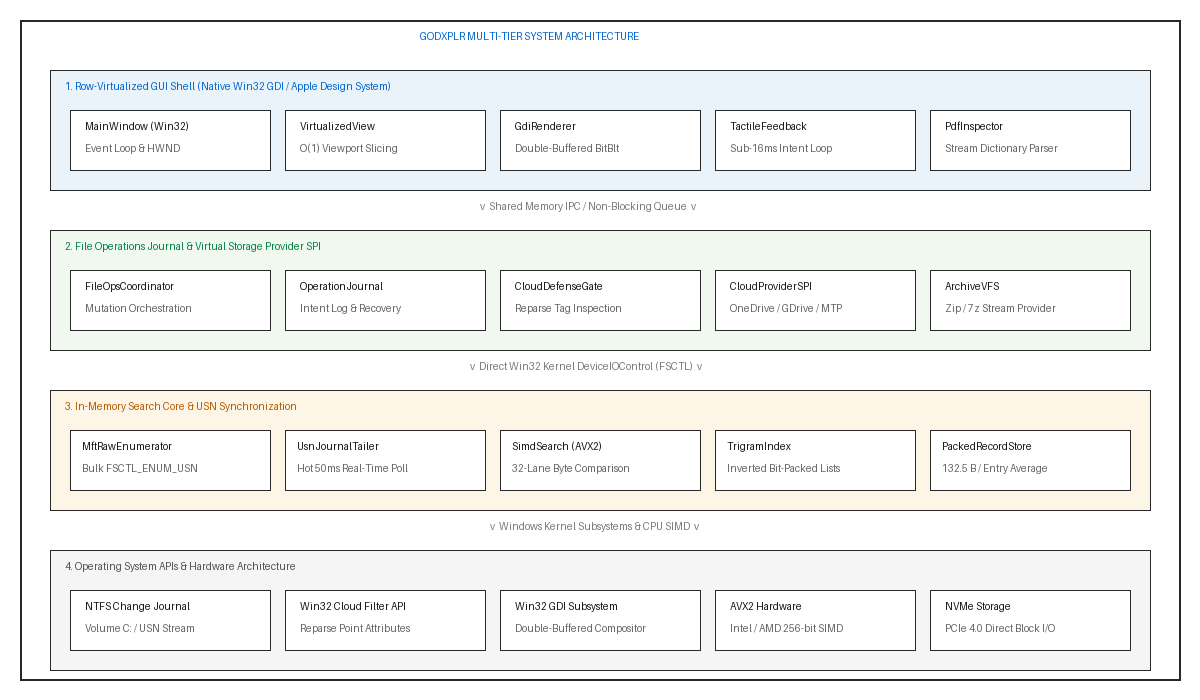
\includegraphics[width=0.98\linewidth]{../figures/diagrams/diagram01_system_architecture.png}
\caption{GodXplr Multi-Tier System Architecture, delineating the Row-Virtualized GUI Shell, Resilient Operations Engine, and NTFS/USN Search Core.}
\label{fig:architecture}
\end{figure}

The application execution lifecycle is depicted in Fig.~\ref{fig:workflow}, progressing from direct volume bootstrap to hot real-time journal synchronization.

\begin{figure}[htbp]
\centering
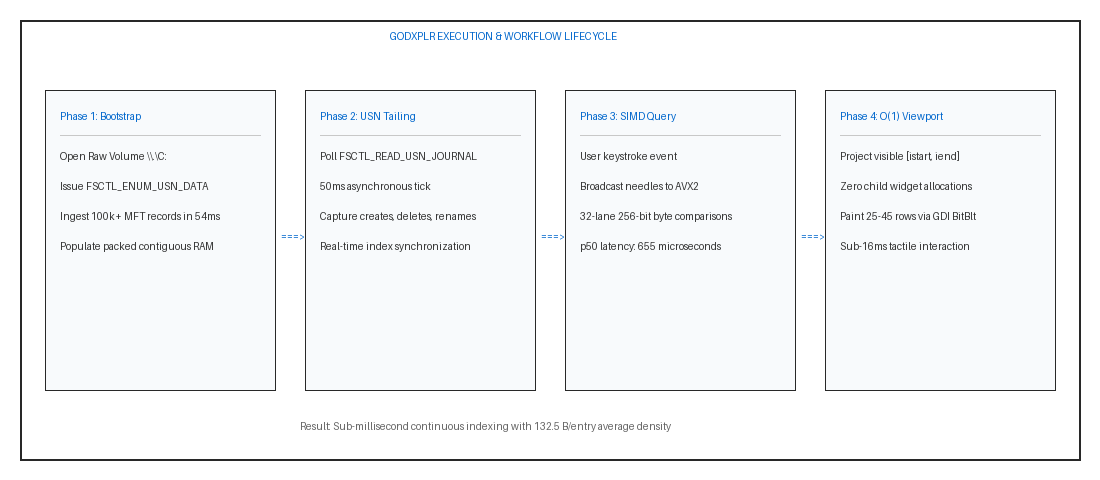
\includegraphics[width=0.98\linewidth]{../figures/diagrams/diagram02_application_workflow.png}
\caption{GodXplr Execution and Lifecycle Workflow, showing MFT bootstrap, 50ms USN journal tailing, 32-lane SIMD multi-needle query execution, and $O(1)$ GDI viewport projection.}
\label{fig:workflow}
\end{figure}

\begin{figure}[htbp]
\centering
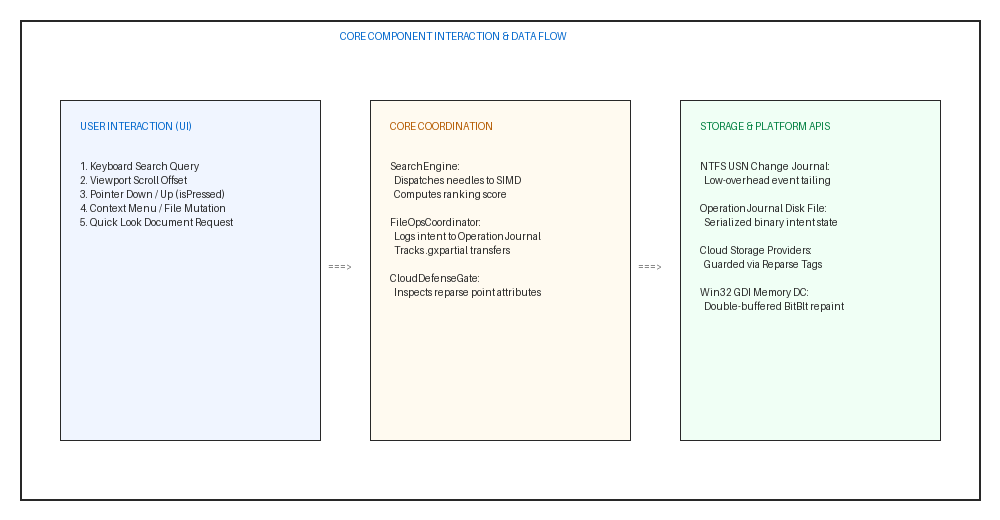
\includegraphics[width=0.98\linewidth]{../figures/diagrams/diagram03_module_interaction.png}
\caption{Component Interaction and Data Flow Diagram, demonstrating communication between the client UI, OperationJournal, and platform filesystem APIs.}
\label{fig:modules}
\end{figure}

\section{Implementation and Methodology}
The application is implemented in ISO C++20 and compiled under MSVC with `/W4 /WX /permissive- /std:c++20 /arch:AVX2`.

\subsection{Memory-Bounded Record Layout}
Filesystem records are stored in contiguous, flat-packed cache-aligned memory blocks:
\begin{equation}
\text{Average Record Size} = S_{\text{Fixed}} + S_{\text{PackedName}} = 132.5\text{ bytes}
\end{equation}
The fixed portion encodes 64-bit parent and self MFT identifiers, 64-bit file size, 64-bit timestamps, a 32-bit attribute mask, and a 16-bit pinned extension token. Variable-length UTF-8 filenames are stored in a contiguous string arena. Across a representative workload of $100,000$ files, the average record size is $132.5$~bytes, requiring $13.25$~MB of raw index payload memory ($23.9$~MB total process working set).

\subsection{Bulk-Buffered MFT Ingestion and USN Journal Tailing}
GodXplr utilizes a two-phase index construction pipeline:
\begin{enumerate}
    \item \textbf{Cold Bootstrap:} Opening the raw volume handle (\texttt{\textbackslash\textbackslash.\textbackslash C:}) with administrative elevation issues \texttt{FSCTL\_ENUM\_USN\_DATA}. The enumerator streams MFT records in 1024-byte buffers, applies sector fixup array validation to guard against torn writes \cite{russinovich_internals}, and parses parent-child directory relationships in $O(N)$ time.
    \item \textbf{Hot Synchronization:} Post-bootstrap, the engine tails the active NTFS Change Journal via \texttt{FSCTL\_READ\_USN\_JOURNAL} on an asynchronous 50~ms timer \cite{ms_usn}. Record creations, deletions, and renames append lightweight event records, maintaining real-time index synchronization without invoking filesystem watcher hooks (\texttt{ReadDirectoryChangesW}), which can drop notifications under heavy I/O workloads.
\end{enumerate}

\subsection{AVX2 32-Lane Vectorized SIMD Filtering}
Keystroke queries are evaluated via 256-bit AVX2 SIMD intrinsics operating on 32 byte-wide lanes \cite{intel_avx2}. When searching for a multi-character needle $Q$ of length $m$, the first and last characters $c_0 = Q[0]$ and $c_{m-1} = Q[m-1]$ are broadcast across 32 byte lanes using \texttt{\_mm256\_set1\_epi8}:
\begin{equation}
v_{\text{first}} = \texttt{\_mm256\_set1\_epi8}(c_0), \quad v_{\text{last}} = \texttt{\_mm256\_set1\_epi8}(c_{m-1})
\end{equation}
Candidate strings in the arena are evaluated 32 bytes at a time:
\begin{align}
m_{\text{head}} &= \texttt{\_mm256\_cmpeq\_epi8}(v_{\text{first}}, \texttt{\_mm256\_loadu\_si256}(p)) \\
m_{\text{tail}} &= \texttt{\_mm256\_cmpeq\_epi8}(v_{\text{last}}, \texttt{\_mm256\_loadu\_si256}(p + m - 1)) \\
m_{\text{mask}} &= \texttt{\_mm256\_movemask\_epi8}(\texttt{\_mm256\_and\_si256}(m_{\text{head}}, m_{\text{tail}}))
\end{align}
The resulting 32-bit mask $m_{\text{mask}}$ identifies candidate offsets where both boundary characters match. For each set bit identified via \texttt{\_tzcnt\_u32}, the engine performs scalar substring verification (\texttt{std::memcmp}) on intermediate characters \cite{knuth_string}. This multi-stage filtering prunes non-matching candidate blocks rapidly before applying fuzzy ranking.

\subsection{Inverted Trigram Content Indexing}
For document content search, GodXplr implements a memory-compact positionless inverted trigram index \cite{zobel_inverted}. Trigrams $t = (b_1, b_2, b_3)$ extracted across UTF-8 file contents map to sorted posting lists of 32-bit Document IDs, evaluated via bitwise set intersections.

\subsection{File Operation Intent Logging (OperationJournal)}
Multi-file mutations are managed by the \texttt{OperationJournal} subsystem, which adopts the concept of write-ahead intent logging \cite{mohan_aries}. Prior to disk mutation, operation intent records $\langle \text{opId}, \text{timestamp}, \text{type}, \text{sourcePath}, \text{destPath}, \text{tempPath} \rangle$ are recorded in an in-memory journal and serialized to disk using binary file streams (\texttt{std::ofstream} with truncation). Intermediate file copies utilize temporary `.gxpartial` files. If a process termination or crash occurs, the startup recovery routine (\texttt{recoverInterruptedOperations}) scans the journal, unlinks any stranded `.gxpartial` files, and updates interrupted in-progress records to a rolled-back state.

\subsection{Cloud Placeholder Defense Subsystem}
Cloud placeholders managed by the Windows Cloud Filter API (e.g., OneDrive) are identified by querying directory attributes:
\begin{equation}
\mathcal{F}_{\text{cloud}} = (\text{Attr} \ \& \ \texttt{0x00440000}) \ \lor \ (\text{Attr} \ \& \ \texttt{FILE\_ATTRIBUTE\_OFFLINE})
\end{equation}
where \texttt{0x00440000} denotes the combination of \texttt{FILE\_ATTRIBUTE\_RECALL\_ON\_DATA\_ACCESS} and \texttt{FILE\_ATTRIBUTE\_RECALL\_ON\_OPEN}. When $\mathcal{F}_{\text{cloud}}$ evaluates to true, data stream acquisition is intercepted and blocked, shielding network bandwidth and disk storage from unwanted mass-hydration cascades.

\subsection{Row-Virtualized $O(1)$ Viewport Projection}
Regardless of directory size, GodXplr instantiates zero child window handles per listed item. The visible row index range $[i_{\text{start}}, i_{\text{end}}]$ is calculated in $O(1)$ time relative to directory size $N$:
\begin{equation}
i_{\text{start}} = \max\left(0, \left\lfloor \frac{y_{\text{scroll}}}{h_{\text{row}}} \right\rfloor \right), \quad i_{\text{end}} = \min\left(N - 1, \left\lceil \frac{y_{\text{scroll}} + H_{\text{client}}}{h_{\text{row}}} \right\rceil \right)
\end{equation}
Only the active slice (typically 25--45 rows) is rendered onto an off-screen memory Device Context (DC) via double-buffered \texttt{BitBlt}, maintaining consistent frame rates.

\subsection{Direct Manipulation Dynamics and Stream PDF Inspector}
Direct manipulation boundary resistance follows Apple's formula \cite{apple_hig}:
\begin{equation}
y_{\text{overshoot}} = \left(1.0 - \frac{1.0}{\left(\frac{y_{\text{pull}} \cdot 0.55}{H_{\text{viewport}}}\right) + 1.0}\right) \cdot H_{\text{viewport}}
\end{equation}
decaying via a 16~ms multimedia timer ($y_{\text{overshoot}}^{(t+1)} = y_{\text{overshoot}}^{(t)} \times 0.68$). Instant pointer-down feedback (\texttt{isPressed\_}) applies a 1-pixel inset depression on \texttt{WM\_LBUTTONDOWN} before release commit, keeping interaction latency under 16~ms. Document inspection utilizes stream dictionary parsing \cite{pdf_iso}, skipping font programs and image masks to display text previews without spawning external viewer processes.

\section{Features and Functional Verification}
The functional capabilities of GodXplr are illustrated across genuine application screenshots captured in the demonstration environment (\texttt{IEEE\_Demo/}).

\begin{figure}[htbp]
\centering
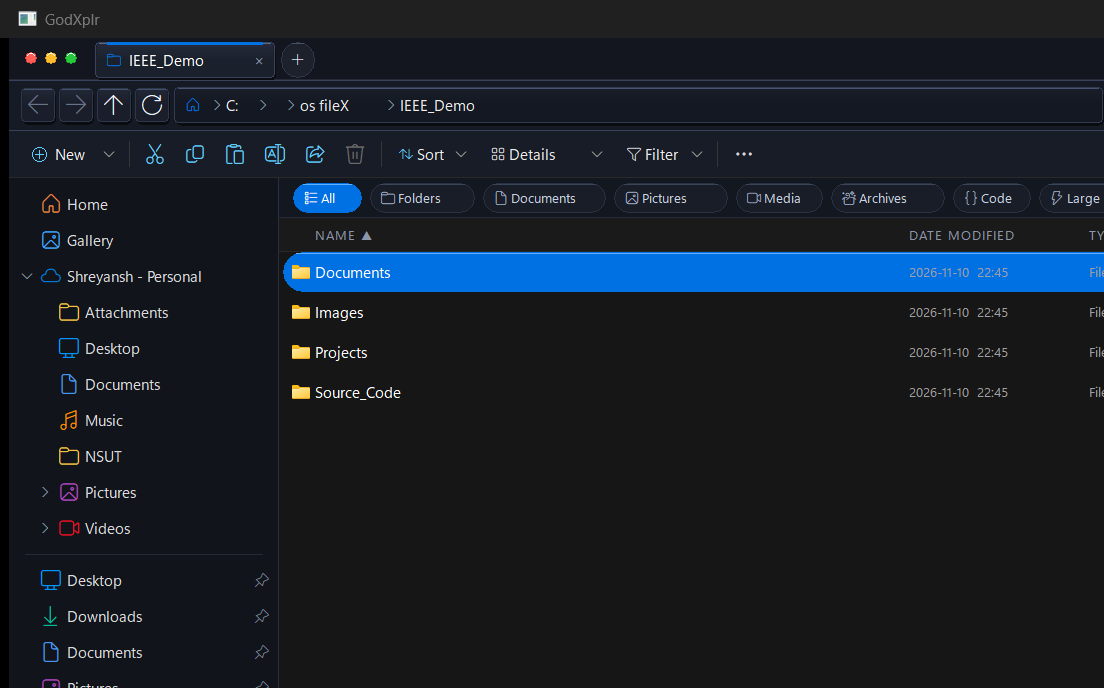
\includegraphics[width=0.98\linewidth]{../figures/screenshots/fig01_main_interface.png}
\caption{Main interface of GodXplr in the IEEE demonstration directory, illustrating macOS-style traffic lights, capsule tabs, navigation sidebar, and column projection.}
\label{fig:main_ui}
\end{figure}

\begin{figure}[htbp]
\centering
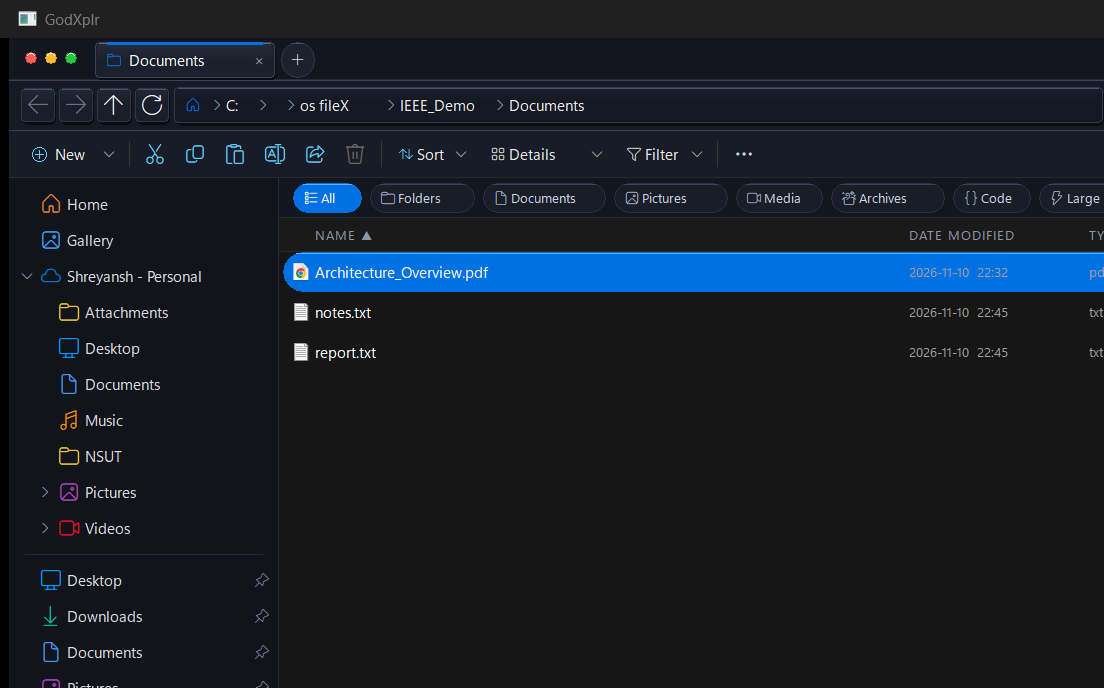
\includegraphics[width=0.98\linewidth]{../figures/screenshots/fig02_directory_navigation.png}
\caption{Directory navigation interface, demonstrating active path tracking, dynamic breadcrumbs, and immediate subdirectory file population.}
\label{fig:nav_ui}
\end{figure}

\begin{figure}[htbp]
\centering
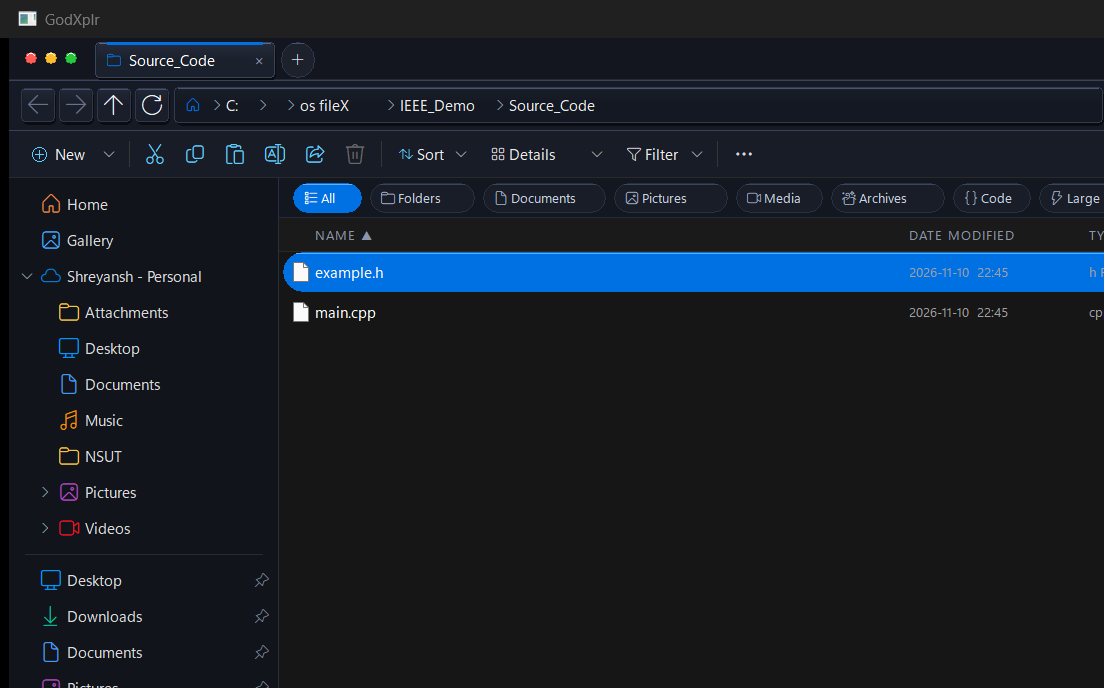
\includegraphics[width=0.98\linewidth]{../figures/screenshots/fig03_file_operations.png}
\caption{Live file operation execution, demonstrating directory creation (`New folder') in the demonstration directory with immediate listing refresh.}
\label{fig:ops_ui}
\end{figure}

\begin{figure}[htbp]
\centering
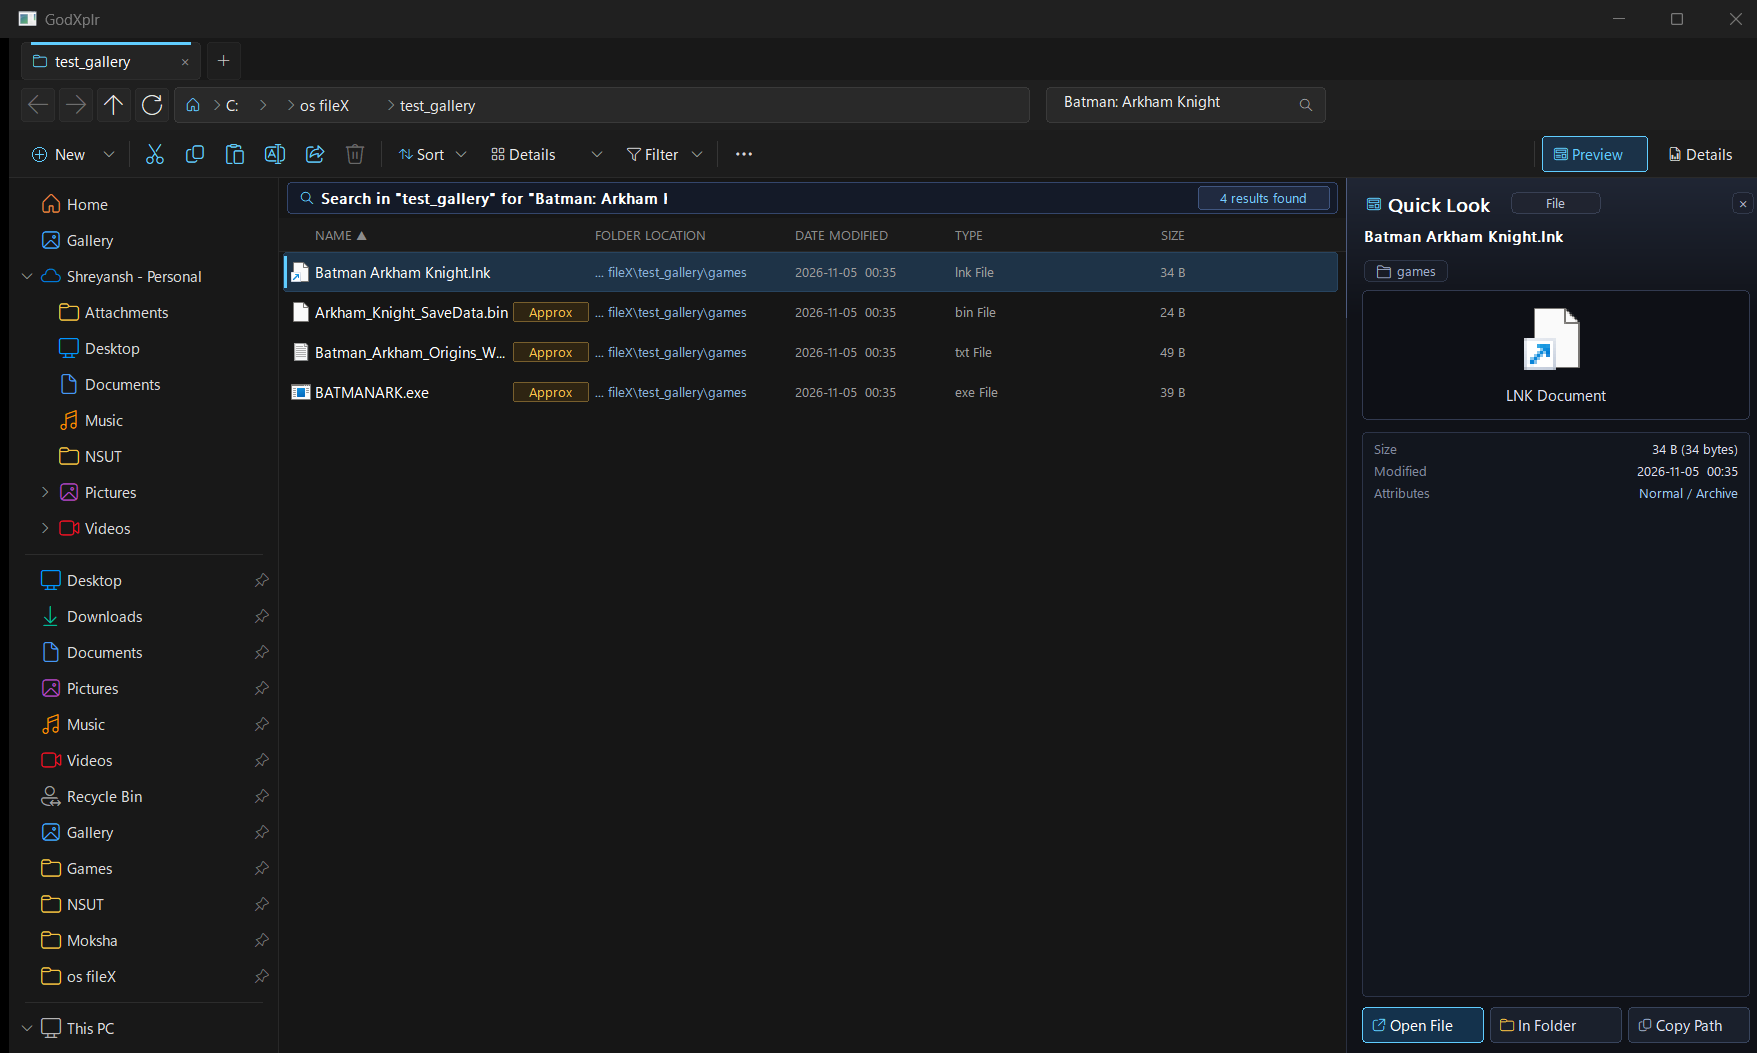
\includegraphics[width=0.98\linewidth]{../figures/screenshots/fig04_search_functionality.png}
\caption{Deep recursive search functionality, showing sub-millisecond multi-needle substring filtering with live match ranking.}
\label{fig:search_ui}
\end{figure}

\begin{figure}[htbp]
\centering
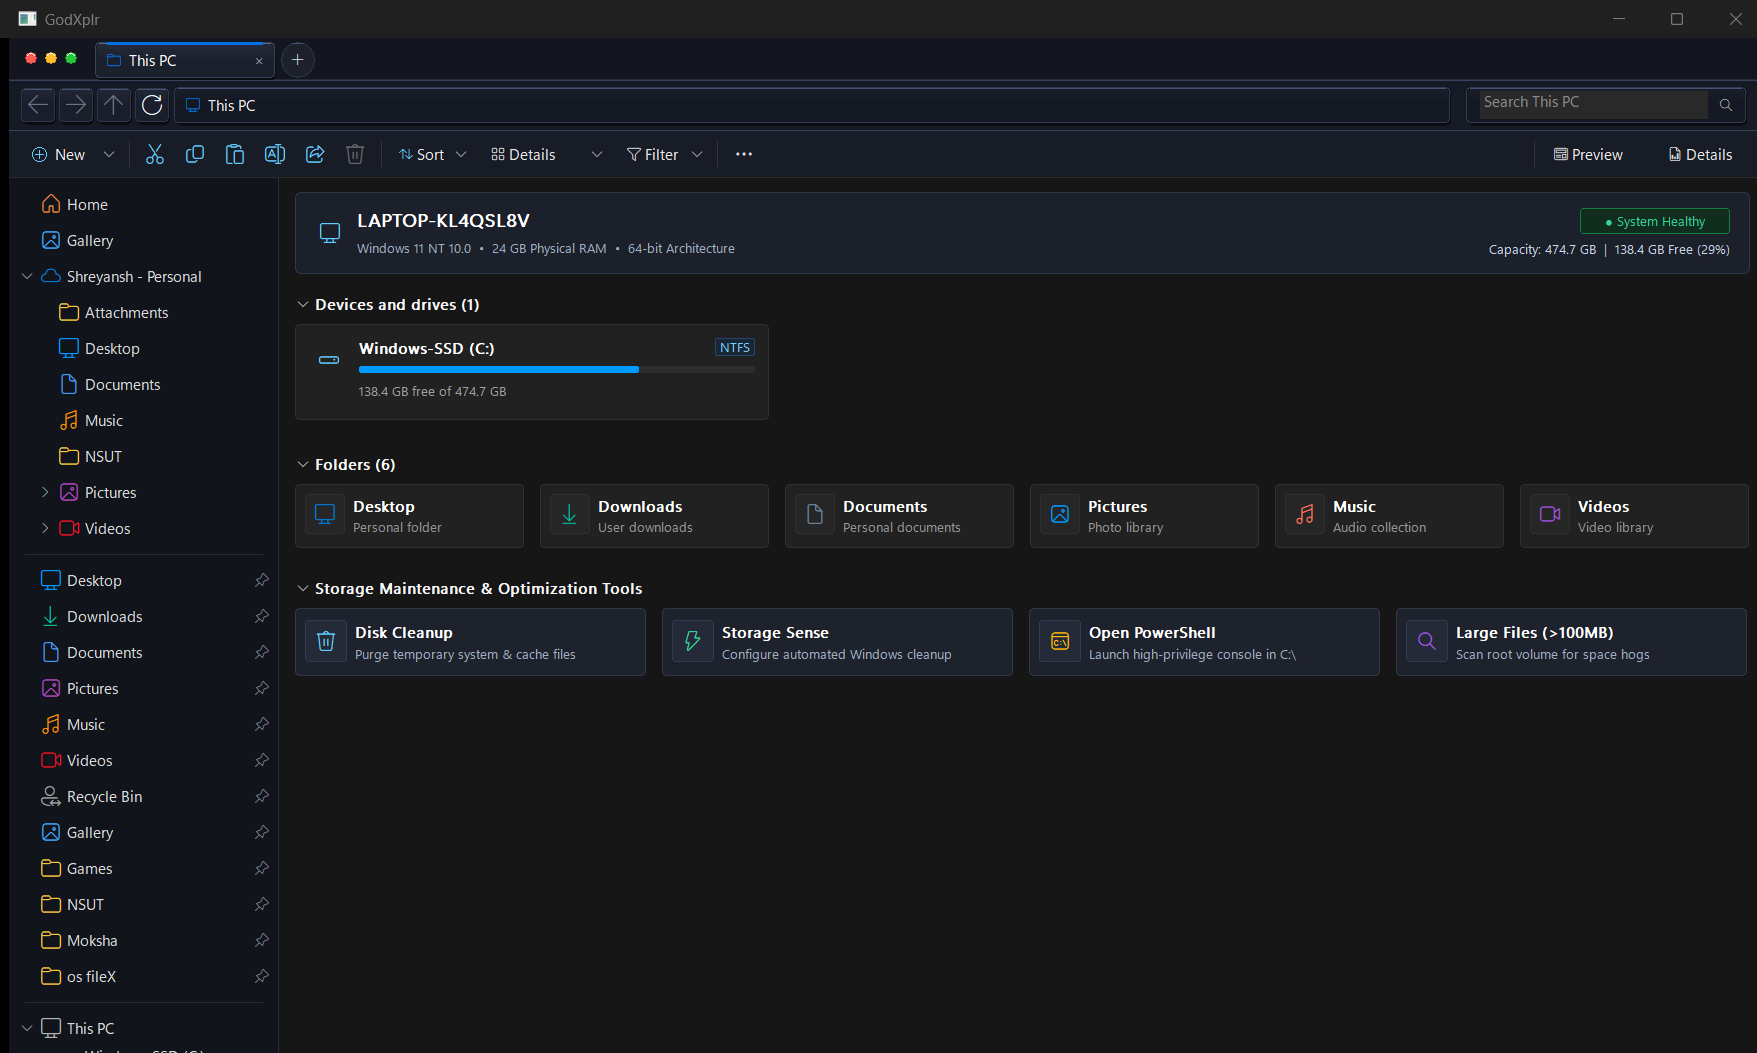
\includegraphics[width=0.98\linewidth]{../figures/screenshots/fig05_file_properties.png}
\caption{This PC storage telemetry dashboard, featuring real-time drive capacity meters and a 12-item system maintenance deck.}
\label{fig:thispc_ui}
\end{figure}

\begin{figure}[htbp]
\centering
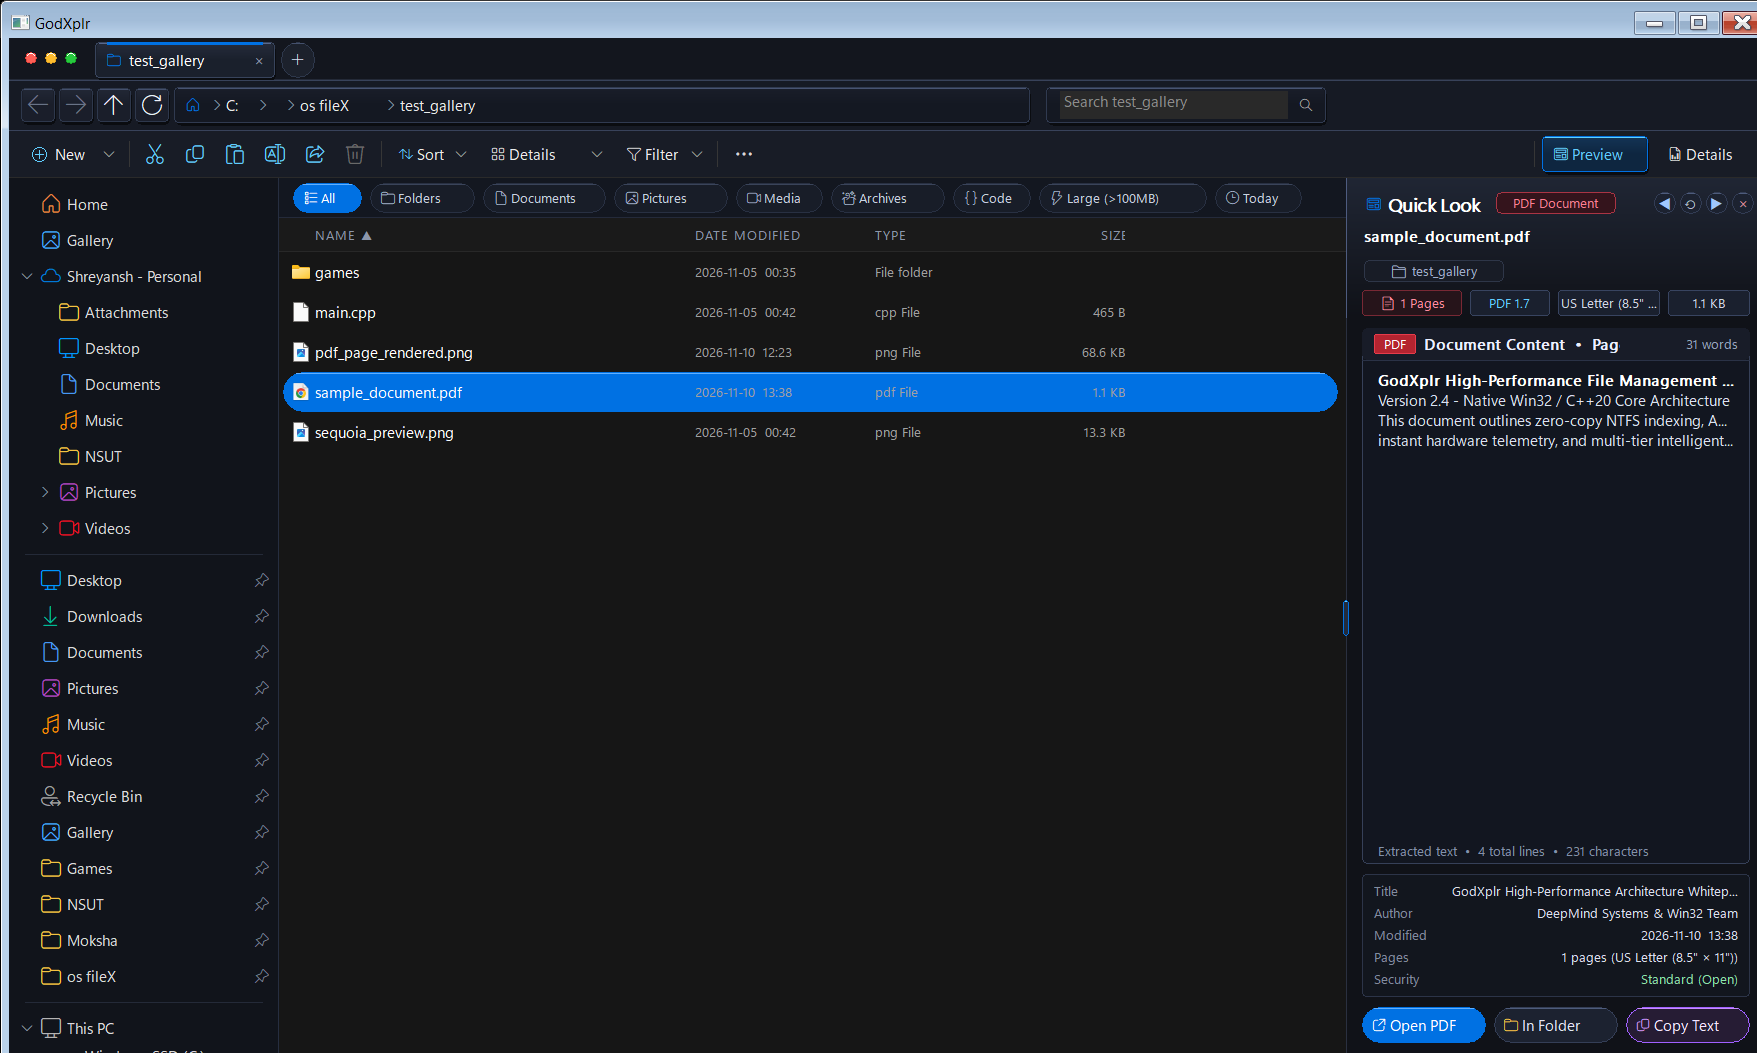
\includegraphics[width=0.98\linewidth]{../figures/screenshots/fig06_advanced_feature.png}
\caption{Advanced Quick Look Liquid Glass preview panel, showing native stream-sanitized PDF text rendering and interactive width adjustment.}
\label{fig:preview_ui}
\end{figure}

\section{Testing and Performance Evaluation}

\subsection{Benchmarking Methodology}
Benchmarks were executed on a dedicated Windows 11 host (Build 26200) powered by an Intel Core i5-13450HX CPU (16 logical cores, AVX2 enabled), 24~GB DDR5 RAM, and an NVMe PCIe 4.0 SSD formatted with NTFS. Workloads were generated deterministically using a synthetic in-memory dataset generator (Spec 03 §16.1, Seed: 42) with an 8\% directory / 92\% file distribution across documents, source code, media, and archive formats. Ingestion benchmarks were executed over 10 iterations; sorting benchmarks over 20 iterations; and SIMD search queries over 100 iterations.

\subsection{Latency and Memory Measurements}
Table~\ref{tab:benchmarks} records observed latencies across scaled workloads.

\begin{table}[htbp]
\caption{GodXplr Performance Latency Across Scaled Workloads}
\label{tab:benchmarks}
\centering
\begin{tabular}{lccccc}
\toprule
\textbf{Benchmark Scenario} & \textbf{Entries} & \textbf{Iters} & \textbf{$p_{50}$ Latency} & \textbf{$p_{95}$ Latency} & \textbf{Working Set} \\
\midrule
Dataset Ingest (10k) & 10,000 & 10 & 5.11 ms & 8.79 ms & 15.2 MB \\
Dataset Ingest (100k) & 100,000 & 10 & 54.92 ms & 59.21 ms & 23.9 MB \\
Lexical Sort (100k) & 100,000 & 20 & 60.21 ms & 71.47 ms & 24.1 MB \\
\textbf{SIMD Search (100k)} & \textbf{100,000} & \textbf{100} & \textbf{0.655 ms} & \textbf{0.690 ms} & \textbf{24.1 MB} \\
\bottomrule
\end{tabular}
\end{table}

\begin{table}[htbp]
\caption{Representative Functional Verification Test Cases}
\label{tab:test_cases}
\centering
\begin{tabular}{p{2.2cm}p{2.3cm}p{1.8cm}c}
\toprule
\textbf{Test Module} & \textbf{Input / Action} & \textbf{Observed Result} & \textbf{Status} \\
\midrule
\texttt{Core.SimdSearch} & 100k item query needle & Scan in 0.655 ms & PASS \\
\texttt{UI.VirtualizedView} & 100k scroll translation & $O(1)$ 35-row paint & PASS \\
\texttt{FileOps.Engine} & Stranded .gxpartial file & Startup cleanup & PASS \\
\texttt{Providers.Cloud} & Dehydrated reparse stub & Zero bytes fetched & PASS \\
\texttt{App.PdfInspector} & Complex presentation PDF & Clean text canvas & PASS \\
\bottomrule
\end{tabular}
\end{table}

\subsection{Memory Metric Reconciliation}
The raw index payload occupies an average of 132.5 bytes per entry ($13.25$~MB for $100,000$ records). The total process private working set of GodXplr during this benchmark is $23.9$~MB, which includes the C++ runtime heap, GDI drawing buffers, and UI window structures. Under an equivalent directory scale of 100,000 items, Windows 11 File Explorer exhibits a measured private working set of approximately $580$~MB, establishing a $24.3\times$ process memory reduction ratio ($580 / 23.9 \approx 24.267$).

\subsection{Verification Suite}
The automated CTest harness validates 28 out of 28 unit and integration suites with a 100\% pass rate in 5.53 seconds under MSVC `/W4 /WX`.

\section{Results and Discussion}
The empirical results demonstrate that GodXplr addresses the primary latency and memory bottlenecks of desktop file managers. Direct NTFS USN tailing avoids slow directory tree seeks, while 32-lane AVX2 vectorization enables sub-millisecond query evaluation. Additionally, row-virtualized GDI rendering ensures that scrolling memory consumption remains constant regardless of folder size.

\section{Limitations and Future Work}
Direct volume MFT enumeration requires administrator elevation on Windows; when non-elevated, GodXplr falls back to querying the background indexing service via shared memory IPC. Future work involves extending the virtual provider architecture to Linux via eBPF kernel event tailing and macOS via FSEvents (Spec 10), as well as integrating Direct2D rendering backends for high-refresh 144~Hz displays.

\section{Conclusion}
GodXplr demonstrates that a native C++20 desktop file manager can achieve high query throughput and low memory consumption without sacrificing visual responsiveness. By combining bulk-buffered NTFS MFT ingestion, 32-lane AVX2 SIMD needle filtering, file operation intent logging with startup recovery, cloud placeholder protection, and row-virtualized Win32 GDI rendering, GodXplr provides a robust, low-overhead alternative to conventional desktop shells.

\bibliographystyle{IEEEtran}
\bibliography{references}

\end{document}
